% Options for packages loaded elsewhere
\PassOptionsToPackage{unicode}{hyperref}
\PassOptionsToPackage{hyphens}{url}
\PassOptionsToPackage{dvipsnames,svgnames,x11names}{xcolor}
%
\documentclass[
  11pt,
  a4paper,
  DIV=11,
  numbers=noendperiod]{scrartcl}

\usepackage{amsmath,amssymb}
\usepackage{iftex}
\ifPDFTeX
  \usepackage[T1]{fontenc}
  \usepackage[utf8]{inputenc}
  \usepackage{textcomp} % provide euro and other symbols
\else % if luatex or xetex
  \usepackage{unicode-math}
  \defaultfontfeatures{Scale=MatchLowercase}
  \defaultfontfeatures[\rmfamily]{Ligatures=TeX,Scale=1}
\fi
\usepackage{lmodern}
\ifPDFTeX\else  
    % xetex/luatex font selection
  \setmainfont[]{Avenir Next}
\fi
% Use upquote if available, for straight quotes in verbatim environments
\IfFileExists{upquote.sty}{\usepackage{upquote}}{}
\IfFileExists{microtype.sty}{% use microtype if available
  \usepackage[]{microtype}
  \UseMicrotypeSet[protrusion]{basicmath} % disable protrusion for tt fonts
}{}
\makeatletter
\@ifundefined{KOMAClassName}{% if non-KOMA class
  \IfFileExists{parskip.sty}{%
    \usepackage{parskip}
  }{% else
    \setlength{\parindent}{0pt}
    \setlength{\parskip}{6pt plus 2pt minus 1pt}}
}{% if KOMA class
  \KOMAoptions{parskip=half}}
\makeatother
\usepackage{xcolor}
\setlength{\emergencystretch}{3em} % prevent overfull lines
\setcounter{secnumdepth}{-\maxdimen} % remove section numbering
% Make \paragraph and \subparagraph free-standing
\ifx\paragraph\undefined\else
  \let\oldparagraph\paragraph
  \renewcommand{\paragraph}[1]{\oldparagraph{#1}\mbox{}}
\fi
\ifx\subparagraph\undefined\else
  \let\oldsubparagraph\subparagraph
  \renewcommand{\subparagraph}[1]{\oldsubparagraph{#1}\mbox{}}
\fi


\providecommand{\tightlist}{%
  \setlength{\itemsep}{0pt}\setlength{\parskip}{0pt}}\usepackage{longtable,booktabs,array}
\usepackage{calc} % for calculating minipage widths
% Correct order of tables after \paragraph or \subparagraph
\usepackage{etoolbox}
\makeatletter
\patchcmd\longtable{\par}{\if@noskipsec\mbox{}\fi\par}{}{}
\makeatother
% Allow footnotes in longtable head/foot
\IfFileExists{footnotehyper.sty}{\usepackage{footnotehyper}}{\usepackage{footnote}}
\makesavenoteenv{longtable}
\usepackage{graphicx}
\makeatletter
\def\maxwidth{\ifdim\Gin@nat@width>\linewidth\linewidth\else\Gin@nat@width\fi}
\def\maxheight{\ifdim\Gin@nat@height>\textheight\textheight\else\Gin@nat@height\fi}
\makeatother
% Scale images if necessary, so that they will not overflow the page
% margins by default, and it is still possible to overwrite the defaults
% using explicit options in \includegraphics[width, height, ...]{}
\setkeys{Gin}{width=\maxwidth,height=\maxheight,keepaspectratio}
% Set default figure placement to htbp
\makeatletter
\def\fps@figure{htbp}
\makeatother

\usepackage[document]{ragged2e}
\KOMAoption{captions}{tableheading}
\makeatletter
\@ifpackageloaded{tcolorbox}{}{\usepackage[skins,breakable]{tcolorbox}}
\@ifpackageloaded{fontawesome5}{}{\usepackage{fontawesome5}}
\definecolor{quarto-callout-color}{HTML}{909090}
\definecolor{quarto-callout-note-color}{HTML}{0758E5}
\definecolor{quarto-callout-important-color}{HTML}{CC1914}
\definecolor{quarto-callout-warning-color}{HTML}{EB9113}
\definecolor{quarto-callout-tip-color}{HTML}{00A047}
\definecolor{quarto-callout-caution-color}{HTML}{FC5300}
\definecolor{quarto-callout-color-frame}{HTML}{acacac}
\definecolor{quarto-callout-note-color-frame}{HTML}{4582ec}
\definecolor{quarto-callout-important-color-frame}{HTML}{d9534f}
\definecolor{quarto-callout-warning-color-frame}{HTML}{f0ad4e}
\definecolor{quarto-callout-tip-color-frame}{HTML}{02b875}
\definecolor{quarto-callout-caution-color-frame}{HTML}{fd7e14}
\makeatother
\makeatletter
\@ifpackageloaded{caption}{}{\usepackage{caption}}
\AtBeginDocument{%
\ifdefined\contentsname
  \renewcommand*\contentsname{Table of contents}
\else
  \newcommand\contentsname{Table of contents}
\fi
\ifdefined\listfigurename
  \renewcommand*\listfigurename{List of Figures}
\else
  \newcommand\listfigurename{List of Figures}
\fi
\ifdefined\listtablename
  \renewcommand*\listtablename{List of Tables}
\else
  \newcommand\listtablename{List of Tables}
\fi
\ifdefined\figurename
  \renewcommand*\figurename{Figure}
\else
  \newcommand\figurename{Figure}
\fi
\ifdefined\tablename
  \renewcommand*\tablename{Table}
\else
  \newcommand\tablename{Table}
\fi
}
\@ifpackageloaded{float}{}{\usepackage{float}}
\floatstyle{ruled}
\@ifundefined{c@chapter}{\newfloat{codelisting}{h}{lop}}{\newfloat{codelisting}{h}{lop}[chapter]}
\floatname{codelisting}{Listing}
\newcommand*\listoflistings{\listof{codelisting}{List of Listings}}
\makeatother
\makeatletter
\makeatother
\makeatletter
\@ifpackageloaded{caption}{}{\usepackage{caption}}
\@ifpackageloaded{subcaption}{}{\usepackage{subcaption}}
\makeatother
\ifLuaTeX
  \usepackage{selnolig}  % disable illegal ligatures
\fi
\usepackage{bookmark}

\IfFileExists{xurl.sty}{\usepackage{xurl}}{} % add URL line breaks if available
\urlstyle{same} % disable monospaced font for URLs
\hypersetup{
  pdftitle={Vererbung},
  colorlinks=true,
  linkcolor={blue},
  filecolor={Maroon},
  citecolor={Blue},
  urlcolor={Blue},
  pdfcreator={LaTeX via pandoc}}

\title{Vererbung}
\author{}
\date{}

\begin{document}
\maketitle

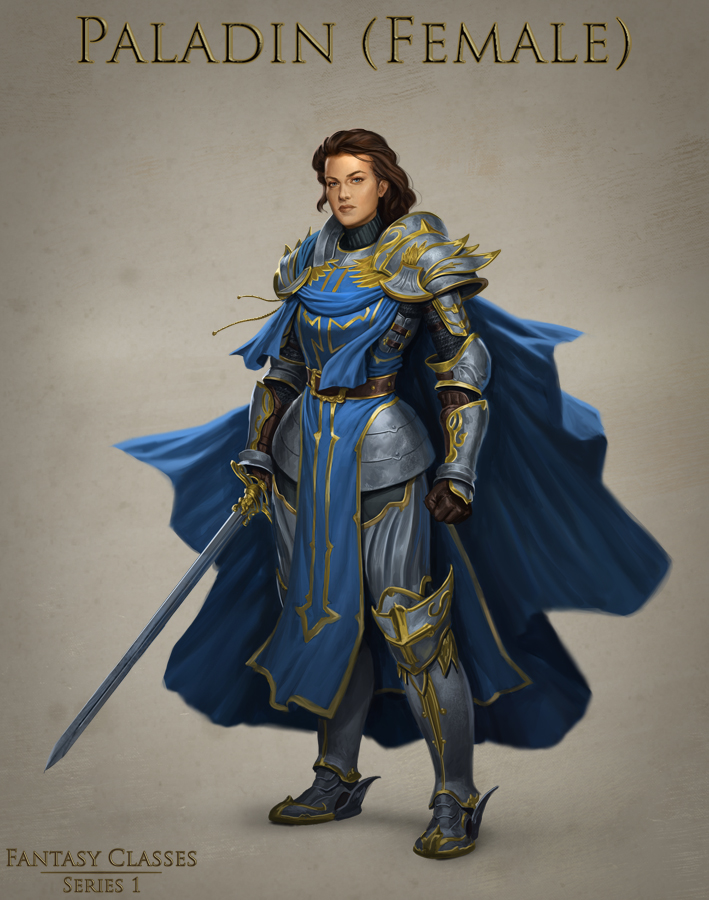
\includegraphics[width=4.16667in,height=\textheight]{/Users/martin/Workspace/Jupyter_Notebooks/Info_KS/2_Objectoriented_Programming/2-3_Inheritance/images/paladin.jpg}

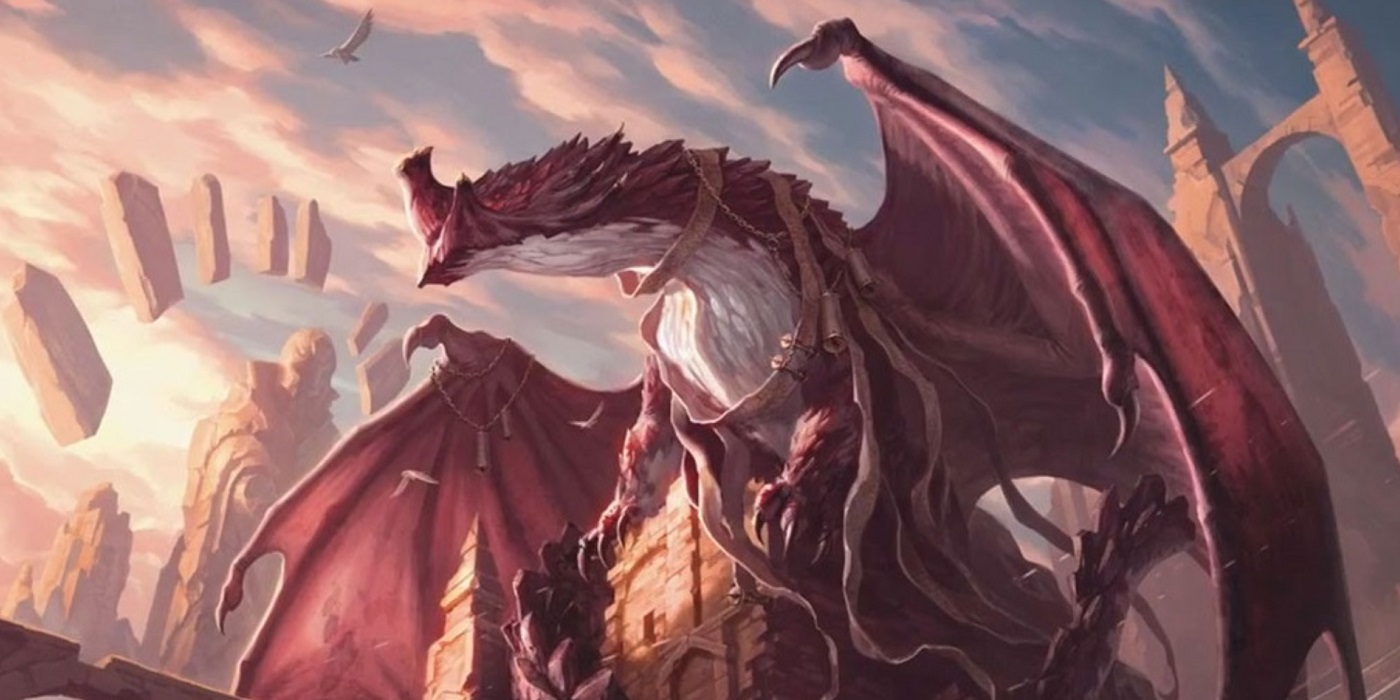
\includegraphics[width=4.16667in,height=\textheight]{/Users/martin/Workspace/Jupyter_Notebooks/Info_KS/2_Objectoriented_Programming/2-3_Inheritance/images/dragon.jpg}

\begin{itemize}
\item
  Es gibt Player Character und Non Player Character.
\item
  Beides sind spezielle Charaktäre, welche gleiche Attribute und gleiche
  Methoden besitzen,
\item
  aber auch unterschiedliche Attribute und Methoden aufweisen können
\item
  Generalisierungshierarchie:
\end{itemize}

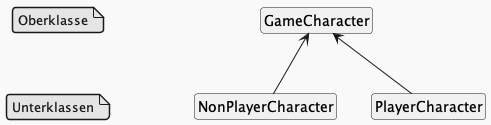
\includegraphics[width=6.25in,height=\textheight]{/Users/martin/Workspace/Jupyter_Notebooks/Info_KS/2_Objectoriented_Programming/2-3_Inheritance/images/classhierarchy.png}

\begin{itemize}
\tightlist
\item
  Terminologie:

  \begin{itemize}
  \tightlist
  \item
    Oberklasse, Superklasse, Elternklasse, Basisklasse
  \item
    Unterklasse, Subklasse, Kindklasse, abgeleitete Klasse.
  \end{itemize}
\item
  Unterklassen erben Atrribute und Methoden der Superklasse
\end{itemize}

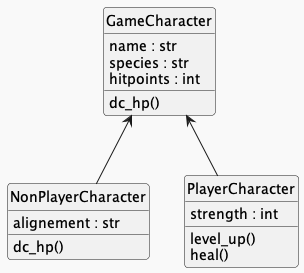
\includegraphics[width=3.125in,height=\textheight]{/Users/martin/Workspace/Jupyter_Notebooks/Info_KS/2_Objectoriented_Programming/2-3_Inheritance/images/classuml.png}

\begin{tcolorbox}[enhanced jigsaw, left=2mm, colframe=quarto-callout-warning-color-frame, opacitybacktitle=0.6, arc=.35mm, toptitle=1mm, colbacktitle=quarto-callout-warning-color!10!white, rightrule=.15mm, colback=white, breakable, toprule=.15mm, bottomtitle=1mm, leftrule=.75mm, titlerule=0mm, bottomrule=.15mm, title=\textcolor{quarto-callout-warning-color}{\faExclamationTriangle}\hspace{0.5em}{Beobachtung}, opacityback=0, coltitle=black]

\begin{itemize}
\tightlist
\item
  gleicher Programmcode wird bei unterschiedlichen Klassen benötigt.
\item
  neues Abstraktionsverfahren wird benötigt: Vererbung
\item
  Code wird an einer Stelle geschreiben, an einer anderen wieder
  verwendet
\end{itemize}

=\textgreater{} Fehlervermeidung

\end{tcolorbox}

\begin{itemize}
\tightlist
\item
  Durch die Vererbung kommen neue Attribute und Methoden hinzu.
\item
  geerbte Methoden können dadurch überschrieben werden \texttt{dc\_hp},
  indem sie in der Subklasse neu definiert werden.
\item
  Beim überschreiben der Methode müssen die Parameter der Methode
  übereinstimmen mit der Methode der Superklasse, kann aber mit weiteren
  Parametern ergänzt werden.
\item
  es wird immer die Methode der Subklassen aufgerufen, wenn sie
  vorhanden ist.
\item
  Beim Methodenaufruf können default-Werte angegeben werden.
  (\texttt{percent:\ int\ =\ 2})
\end{itemize}



\end{document}
